\chapter{Classical Statistical Models}
\label{ch:classical}

This chapter presents the classical time series modeling pipeline implemented in \texttt{02\_classical\_models\_claude.ipynb}. The approach establishes defensible baselines, maps where univariate structure exists in the panel, and produces per-series winner tables for potential ensemble use.

\section{Motivation for Classical Baselines}

Classical models are not expected to win overall against global ML models that can exploit the 86 anonymized features and cross-series structure. However, they serve four essential purposes:

\begin{enumerate}
    \item \textbf{Establish a defensible floor.} If machine learning cannot beat the Naive forecast, something fundamental is broken in the ML pipeline.
    \item \textbf{Map univariate structure.} Per-horizon and per-sub-category breakdowns reveal which parts of the panel have genuine serial structure versus noise.
    \item \textbf{Feed ensemble strategies.} Per-series winner tables can be used by ensemble notebooks to select the best univariate model per series.
    \item \textbf{Honor the EDA.} The 100\% stationarity result from the ADF analysis (Section~\ref{sec:stationarity}) is a load-bearing claim that directly shapes model specifications.
\end{enumerate}

\section{Evaluation Metrics}

Every (series, model) pair is scored with four metrics:

\begin{enumerate}
    \item \textbf{Weighted Skill Score:} The competition metric (Equation~\ref{eq:skill_score}).
    \item \textbf{Weighted RMSE:} $\sqrt{\frac{\sum w_i (y_i - \hat{y}_i)^2}{\sum w_i}}$ --- raw-scale error.
    \item \textbf{Weighted MAE:} $\frac{\sum w_i |y_i - \hat{y}_i|}{\sum w_i}$ --- robust to outliers.
    \item \textbf{MASE (Mean Absolute Scaled Error):} $\frac{\text{mean}(|y_i - \hat{y}_i|)}{\text{mean}(|\Delta y_{\text{train}}|)}$ --- scale-independent, comparable across series with different target magnitudes.
\end{enumerate}

\section{Model Lineup}

The classical modeling notebook evaluates \textbf{41 model specifications} across 6 families. All parametric families use first differencing ($d = 1$), honoring the EDA's stationarity finding.

\subsection{Family A: Baselines (on Levels)}

These models involve no fitting and no differencing. They measure how much of the scored metric is explainable by trivial rules.

\begin{table}[H]
\centering
\caption{Baseline model specifications.}
\begin{tabular}{lp{8cm}}
\toprule
\textbf{Model} & \textbf{Description} \\
\midrule
Zero & $\hat{y}_{t+h} = 0$ for every step. The skill score denominator is exactly the squared error of this forecast. \\
Naive & $\hat{y}_{t+h} = y_t$ (last observed value). Wins when lag-1 autocorrelation is large. \\
Drift & $\hat{y}_{t+h} = y_t + h \cdot \text{slope}$, where slope $= (y_t - y_1)/(n-1)$. Linear extrapolation. \\
Expanding Mean & $\hat{y}_{t+h} = \frac{1}{t}\sum y_i$. Long-run average; wins on mean-reverting series. \\
Rolling Mean ($w=10$) & Mean of the last 10 observations. Local mean, smoother than Naive. \\
\bottomrule
\end{tabular}
\end{table}

\subsection{Family B: AR Family (First Differences)}

An AR($p$) model writes the current differenced value as a linear combination of the previous $p$ differenced values:

\begin{equation}
\Delta y_t = c + \phi_1 \Delta y_{t-1} + \phi_2 \Delta y_{t-2} + \cdots + \phi_p \Delta y_{t-p} + \varepsilon_t
\end{equation}

This is implemented as ARIMA($p$, 1, 0). The parameter $p$ represents memory depth: AR(1) says ``only yesterday matters,'' while AR(10) says ``the last ten days jointly matter.''

\textbf{Lineup:} AR(1) through AR(10), all on first differences.

\textbf{Strengths:} Computationally cheap, interpretable, optimal when the true data-generating process is linear in its own past.

\textbf{Weaknesses:} Cannot model nonlinearity (regime changes, volatility clustering). Higher $p$ increases overfitting risk on short series.

\subsection{Family C: MA Family (First Differences)}

An MA($q$) model says the current differenced value is a linear combination of the last $q$ innovations (random shocks):

\begin{equation}
\Delta y_t = c + \varepsilon_t + \theta_1 \varepsilon_{t-1} + \theta_2 \varepsilon_{t-2} + \cdots + \theta_q \varepsilon_{t-q}
\end{equation}

Implemented as ARIMA(0, 1, $q$). Notably, MA(1) on differences is equivalent to Simple Exponential Smoothing.

\textbf{Lineup:} MA(1) through MA(10), mirroring the AR scan.

\subsection{Family D: ARMA Family (First Differences)}

ARMA combines both channels---past values AND past shocks:

\begin{equation}
\Delta y_t = c + \sum_{i=1}^{p} \phi_i \Delta y_{t-i} + \sum_{j=1}^{q} \theta_j \varepsilon_{t-j} + \varepsilon_t
\end{equation}

Implemented as ARIMA($p$, 1, $q$) with both $p \geq 1$ and $q \geq 1$.

\textbf{Lineup:} 10 variants covering $(p,q)$ combinations from ARMA(1,1) to ARMA(4,4), with total order $p+q$ ranging from 2 to 8.

\subsection{Family E: ARIMA with Explicit $d$ Comparison}

This family includes both $d = 0$ and $d = 1$ variants to enable a matched-pair head-to-head comparison:

\begin{table}[H]
\centering
\caption{ARIMA variants for the $d=0$ vs. $d=1$ comparison.}
\begin{tabular}{ll}
\toprule
\textbf{Model} & \textbf{Purpose} \\
\midrule
ARIMA(0,1,0) & Pure random walk baseline \\
ARIMA(1,0,0) & AR(1) on levels ($d=0$ contrast) \\
ARIMA(1,0,1) & ARMA(1,1) on levels ($d=0$ contrast) \\
ARIMA(2,0,2) & ARMA(2,2) on levels ($d=0$ contrast) \\
\bottomrule
\end{tabular}
\end{table}

If the EDA's stationarity claim is correct, the $d=1$ variants should systematically outperform their $d=0$ counterparts.

\subsection{Family F: SARIMA}

SARIMA($p, d, q$)($P, D, Q, s$) adds seasonal AR, differencing, and MA terms with period $s$:

\begin{equation}
\Phi(B^s)\, \phi(B)\, (1-B)^d\, (1-B^s)^D\, y_t = \Theta(B^s)\, \theta(B)\, \varepsilon_t
\end{equation}

Two variants are included:
\begin{itemize}
    \item SARIMA(1,1,1)(1,1,1,7) --- weekly-length cycle
    \item SARIMA(1,1,1)(1,1,1,24) --- daily-length cycle
\end{itemize}

Given the absence of panel-wide seasonality in the EDA, SARIMA is included for completeness rather than expectation of strong performance.

\section{Evaluation Design}

\subsection{Eligibility and Splitting}

A series is eligible if it crosses $\texttt{VAL\_CUTOFF} = 2880$. The temporal split is strict: training uses $\texttt{ts\_index} \leq 2880$, validation uses $\texttt{ts\_index} > 2880$.

\begin{figure}[H]
\centering
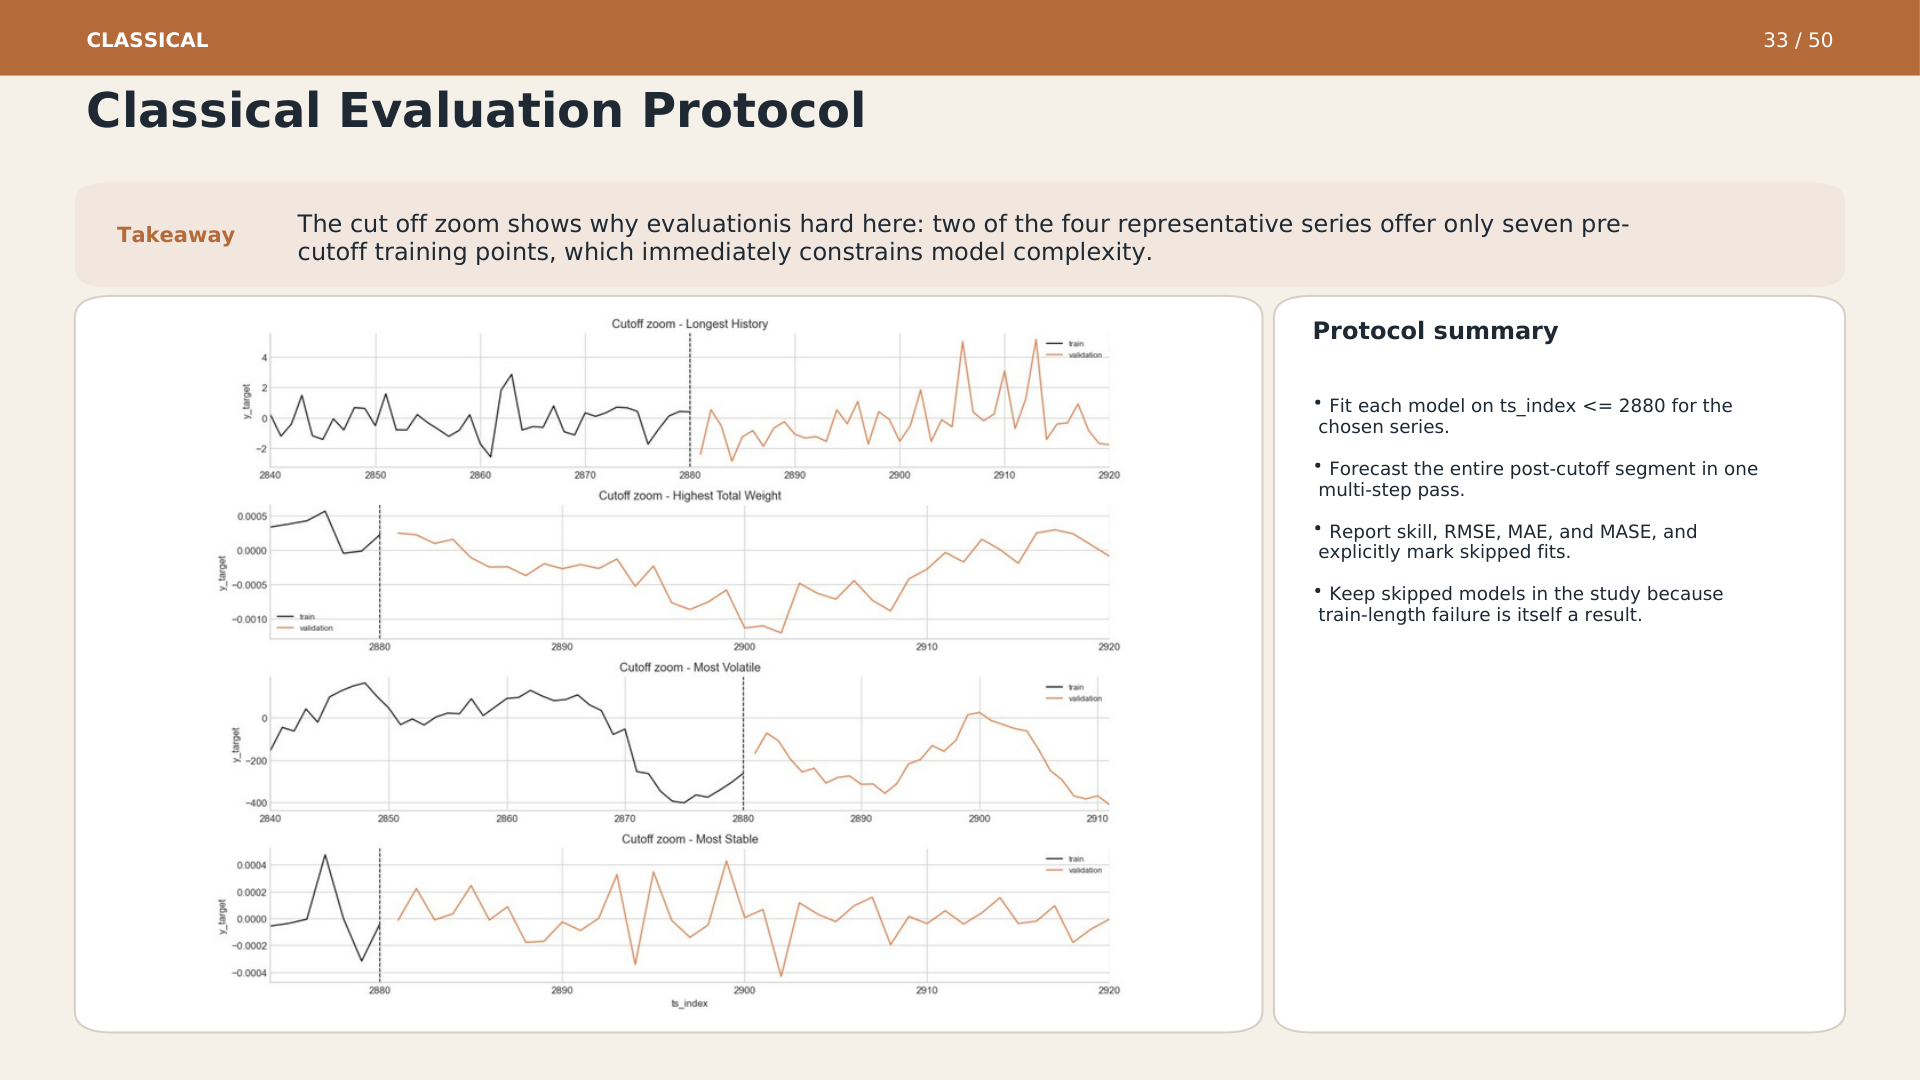
\includegraphics[width=0.95\textwidth]{figures/slide_30.png}
\caption{Classical evaluation protocol. The cutoff zoom reveals the challenge: four representative series around the $\texttt{ts\_index} = 2880$ boundary show vastly different scales and behaviors. Two of the four have only seven pre-cutoff training points, which immediately constrains model complexity.}
\label{fig:classical_eval}
\end{figure}

\subsection{Skip and Failure Handling}

Each model specification has a \texttt{min\_train} parameter. If a series has fewer training observations than this threshold, the (series, model) pair is marked as ``skipped.'' If a model's fit raises an exception or produces non-finite values, it is marked as ``failed.'' Both conditions are tracked and reported.

\subsection{Sample Run Results}

Running on a sample of 200 eligible series (out of 1,930) with 41 models produces 8,200 (series, model) evaluation rows:

\begin{table}[H]
\centering
\caption{Status distribution for the sample run (200 series $\times$ 41 models).}
\begin{tabular}{lr}
\toprule
\textbf{Status} & \textbf{Count} \\
\midrule
ok & 6,735 \\
skipped & 1,464 \\
failed & 1 \\
\midrule
Total & 8,200 \\
\bottomrule
\end{tabular}
\end{table}

The high skip rate (17.9\%) is driven primarily by SARIMA models, which require longer training histories, and by higher-order AR/MA/ARMA models on short series.

\section{Key Insights from Classical Modeling}

\subsection{Leaderboard Results}

The per-model leaderboard (aggregating across all evaluated series) reveals several patterns:

\begin{enumerate}
    \item \textbf{Baselines are surprisingly competitive.} The Expanding Mean and Rolling Mean models often perform comparably to or better than fitted parametric models, reflecting the difficulty of beating simple forecasts on noisy financial data.
    \item \textbf{Low-order models tend to outperform high-order ones.} AR(1)--AR(3) generally outperform AR(7)--AR(10), consistent with the ACF analysis showing short-lag dominance.
    \item \textbf{MA(1) on differences is strong.} As the mathematical equivalent of Simple Exponential Smoothing, MA(1) is a robust performer.
\end{enumerate}

\subsection{The $d=0$ vs. $d=1$ Head-to-Head}

Comparing matched-order ARIMA pairs confirms the EDA's stationarity finding:
\begin{itemize}
    \item ARIMA($p$, 1, $q$) variants systematically outperform their ARIMA($p$, 0, $q$) counterparts.
    \item First differencing is genuinely load-bearing for this dataset.
\end{itemize}

\subsection{Per-Series Winner Analysis}

No single model dominates across all series. The per-series winner table shows considerable heterogeneity:
\begin{itemize}
    \item Some series are best served by simple baselines (Naive, Expanding Mean).
    \item Others benefit from low-order AR or MA models.
    \item Very few series favor high-order ARMA or SARIMA specifications.
\end{itemize}

This heterogeneity motivates ensemble approaches that select or blend models per-series.

\section{Limitations of Classical Models}

\begin{enumerate}
    \item \textbf{Univariate only:} Classical models cannot exploit the 86 predictor features.
    \item \textbf{Linear assumptions:} AR/MA/ARMA/ARIMA assume linear relationships, missing nonlinear dynamics.
    \item \textbf{No cross-series learning:} Each series is modeled independently, ignoring potential shared structure across the panel.
    \item \textbf{Computational cost at scale:} Fitting 41 models on 1,930 series requires significant computation.
\end{enumerate}

These limitations motivate the deep learning approach in the next chapter.
